\section{Application 1: Whitened Variational Gaussian Processes}
\label{sec:variational_results}

As a first application of the CIQ method, we will demonstrate that the scalable whitening procedure $\bK^{-1/2} \bb$ can accelerate and increase the fidelity of variational Gaussian process approximations \cite{hensman2013gaussian,hensman2015scalable,matthews2017scalable}.
The whitening operation is commonly used with variational approximations to accelerate the learning of variational parameters \cite{matthews2017gpflow}.


\paragraph{Whitened Stochastic Variational Gaussian Processes.}
Stochastic variational Gaussian processes (SVGP) are used when the data are modelled with non-conjugate likelihoods (e.g. classification) or for large datasets that might not fit into memory.
Recall from \cref{sec:variational} that these models form an approximate predictive distribution
\[
  p(f(\bx) \mid \bX, \by) \approx \Evover{q(\bu)}{ p\left( f(\bx) \mid \bu \right)} = \normaldist{ \bxtest; \ameantest{ \bx }} { \avartest{ \bx }},
\]
where $q \left( \bu \right)$ is a Gaussian distribution parameterized by mean $\bm \in \reals^M$ and covariance $\bS \in \reals^{M \times M}$.
$\bm$ and $\bS$ (as well as inducing point locations $\bZ$ and kernel/likelihood hyperparameters) are chosen to optimizing the variational ELBO (\cref{eqn:elbo}):
%
\begin{align*}
	-\loglik_\text{ELBO} &= -\sum_{i=1}^N \Evover{q(f(\bx^{(i)}))}{  \: \log p( y^{(i)} \mid f(\bx^{(i)}) ) \: } + \kl{ q(\bu) }{ p(\bu) }.
\end{align*}
%
As stated in \cref{sec:variational}, the ELBO factorizes over all data points in the training set $\bX, \by$.
Therefore, it can be approximated using minibatches and used in conjunction with stochastic gradient optimization.

Rather than directly learning $\bm$ and $\bS$, it is more common to learn the \emph{whitened parameters} \cite{kuss2005assessing,matthews2017scalable}:
\[ \bm' = \bK^{-\frac 1 2} \bm, \quad \bS' = \bK^{-\frac 1 2} \bS \bK^{-\frac 1 2} \]
Under this coordinate system, the KL divergence term is given by
%
\begin{equation}
	\kl{ q(\bu') }{ p(\bu') } = \frac{1}{2} \Bigl( \bm^{\prime \top} \bm' + \tr{ \bS' } - \log \vert \bS' \vert - M \Bigr),
	\label{eqn:kldiv_whitened}
\end{equation}
%
which, importantly, doesn't depend on $k(\cdot,\cdot)$ or $\bZ$ and therefore is relatively simple to optimize.
With whitening, the predictive mean and variance of become:
%
\begin{align}
  \ameantest{\bx} &= \bk_{\bZ\bx}^\top \bK^{-\frac 1 2} \bm'
  \label{eqn:approx_pred_mean} \\
  \avartest{\bx} &= k(\bx, \bx) -
    \bk_{\bZ\bx}^\top \bK^{-\frac 1 2} \left( \bI - \bS' \right) \bK^{-\frac 1 2} \bk_{\bZ\bx}
  \label{eqn:approx_pred_covar}
\end{align}
%
During training, we repeatedly compute the ELBO and its derivative when performing stochastic gradient optimization.
At each iteration, we must compute \cref{eqn:approx_pred_mean,eqn:approx_pred_covar} for a minibatch of data points $\bx_i$.
Optimization typically requires up to $10,\!000$ iterations of training \citep[e.g.][]{salimbeni2018natural};
therefore, we must compute $\bK^{- \frac 1 2} \bk_{\bX \bx_i}$ and its derivative \emph{thousands of times} over the course of training.

\gp{Stopped here.}

\begin{figure}[t!]
  \centering
  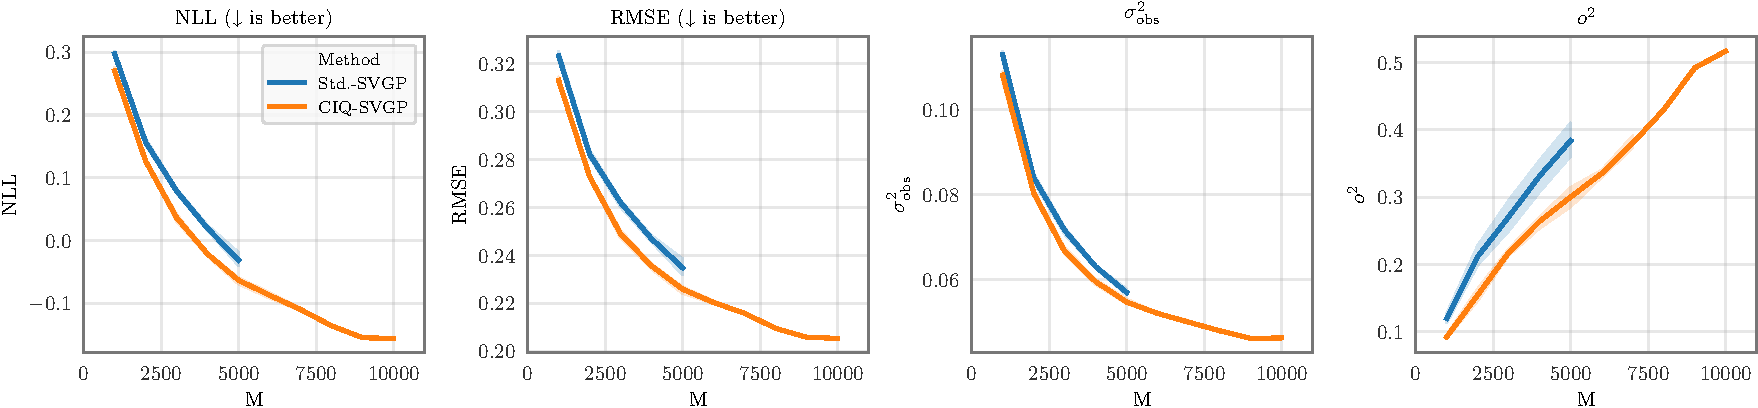
\includegraphics[width=\linewidth]{figures/3droad.pdf}
  \caption{
    SVGP models trained on the 3D-Road dataset ($D=2$, $N\geq300,\!000$), varying $M$ (the number of inducing points).
    \gp{FINISH}
  }
  \label{fig:3droad}
\end{figure}

\begin{figure}[t!]
  \centering
  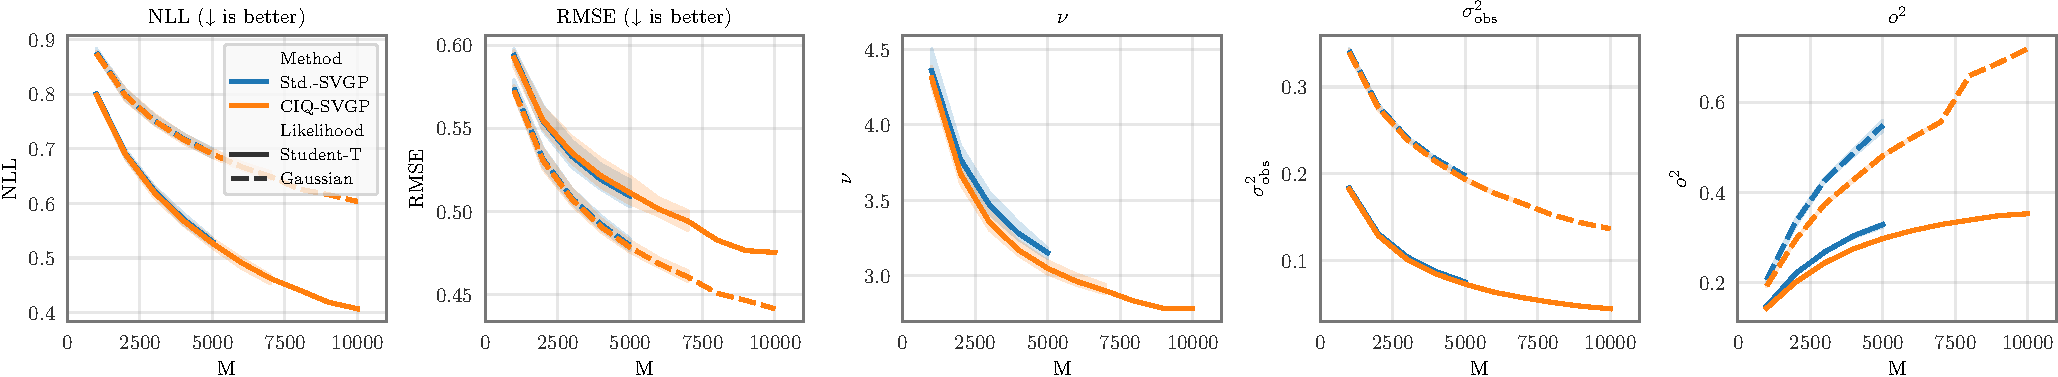
\includegraphics[width=\linewidth]{figures/precip.pdf}
  \caption{
    SVGP models trained on the Precipitation dataset ($D=3$, $N\geq300,\!000$), varying $M$ (the number of inducing points).
    \gp{FINISH}
  }
  \label{fig:precip}
\end{figure}

\begin{figure}[t!]
  \centering
  \caption{
    SVGP models trained on the Robotics dataset ($D=?$, $N\geq?$), varying $M$ (the number of inducing points).
    \gp{FINISH}
  }
  \label{fig:robotics}
\end{figure}
